\documentclass[11pt,a4paper,twoside,titlepage]{article}
\usepackage{float}
\usepackage{lipsum}
\usepackage[utf8]{inputenc}
\usepackage{blindtext}
\usepackage[margin=0.75in,top=1.1in,bottom=0.75in]{geometry}
\usepackage[normalem]{ulem}
\usepackage{graphicx}  
\usepackage{eqnarray,amsmath,amsthm}
\usepackage[final]{pdfpages}
\usepackage[version=4]{mhchem}
\usepackage{hyperref}
\usepackage{pdflscape}
\usepackage{longtable,booktabs}
\usepackage{cite}
\usepackage{gensymb}
\usepackage{parskip}
\usepackage{fancyhdr}
\usepackage[numbib]{tocbibind}
\usepackage{multicol}
\usepackage{caption}
\usepackage{subcaption}
\usepackage{listings}
\usepackage{color} %red, green, blue, yellow, cyan, magenta, black, white
\definecolor{mygreen}{RGB}{28,172,0} % color values Red, Green, Blue
\definecolor{mylilas}{RGB}{170,55,241}
\lstset{language=Matlab,%
    %basicstyle=\color{red},
    breaklines=true,%
    morekeywords={matlab2tikz},
  %  basicstyle=10pt,       				% the size of the fonts that are used for the code
    frame=single,	                			% adds a frame around the code
    keywordstyle=\color{blue},%
    morekeywords=[2]{1}, keywordstyle=[2]{\color{black}},
    identifierstyle=\color{black},%
    stringstyle=\color{mylilas},
    commentstyle=\color{mygreen},%
    showstringspaces=false,%without this there will be a symbol in the places where there is a space
    numbers=left,%
    numberstyle={\tiny \color{black}},% size of the numbers
    numbersep=9pt, % this defines how far the numbers are from the text
    emph=[1]{for,end,break},emphstyle=[1]\color{red}, %some words to emphasise
    %emph=[2]{word1,word2}, emphstyle=[2]{style},    
}

\renewcommand*\contentsname{Table of Contents}
\begin{document}
\begin{titlepage}
  \begin{center}
    
\includegraphics[width=1in]{fig/Universitaet_Logo_RGB.pdf}\\
    \line(2,0){375}\\
    [3.5mm]
    \textbf{\Large{TECHNISCHE UNIVERSITÄT MÜNCHEN}} \\
    \large{\textbf{FAKULTÄT FÜR INFORMATIK}}\\
    \line(1,0){300}\\
    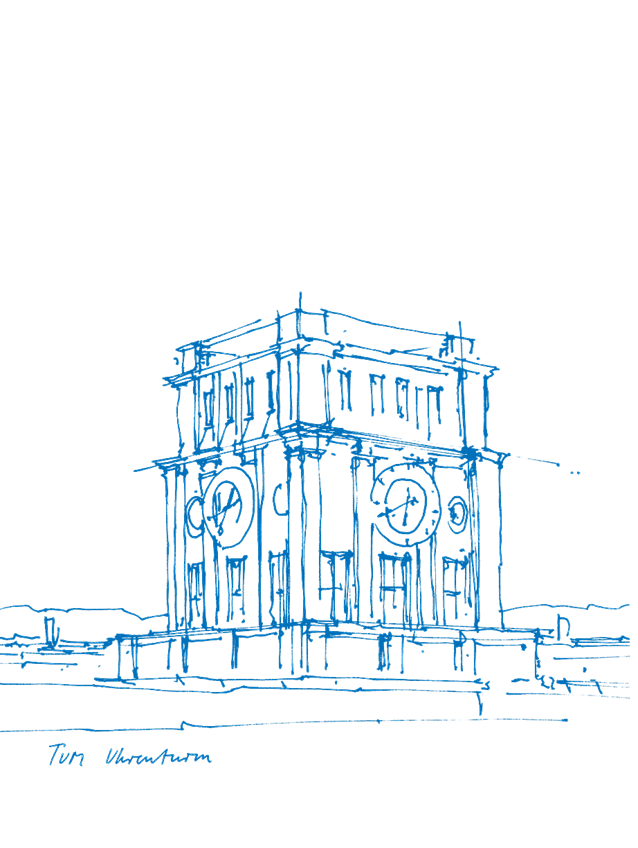
\includegraphics[width=5in,height=15cm,keepaspectratio]{fig/TUM_Uhrenturm.png}\\[1cm]
    \Large{\textbf {NAME OF LECTURE}} \\[0.5cm]
    \Large{\textbf {LECTURE NOTES}}
  \end{center}
  \begin{flushleft}
    \vspace{2cm}
    \begin{tabular}{ l l l }
      \textbf {Written by:} &  & Muhammed Kürşat Yurt \\
    \end{tabular}
  \end{flushleft}
\end{titlepage}
\pagestyle{fancy}
\fancyhf{}
\renewcommand{\headrulewidth}{1.75pt}
\renewcommand{\footrulewidth}{1.5pt}
\fancyfoot[C]{\thepage}
\renewcommand{\sectionmark}[1]{\markright{#1}}
\fancyhead[C]{\textbf{\MakeUppercase{\rightmark}}}
\pagenumbering{roman}
\newpage
\tableofcontents
\newpage
\pagenumbering{arabic}
\setcounter{page}{1}

\section{Introduction}

xx

\section{Section 2}
xx
\subsection{Subsec 1 }
xx
\subsection{Subsec 2}
\end{document}
